\clearpage
\newpage
\section*{Extend data figures}

\setcounter{figure}{0}

\begin{figure}[ht]
\centering
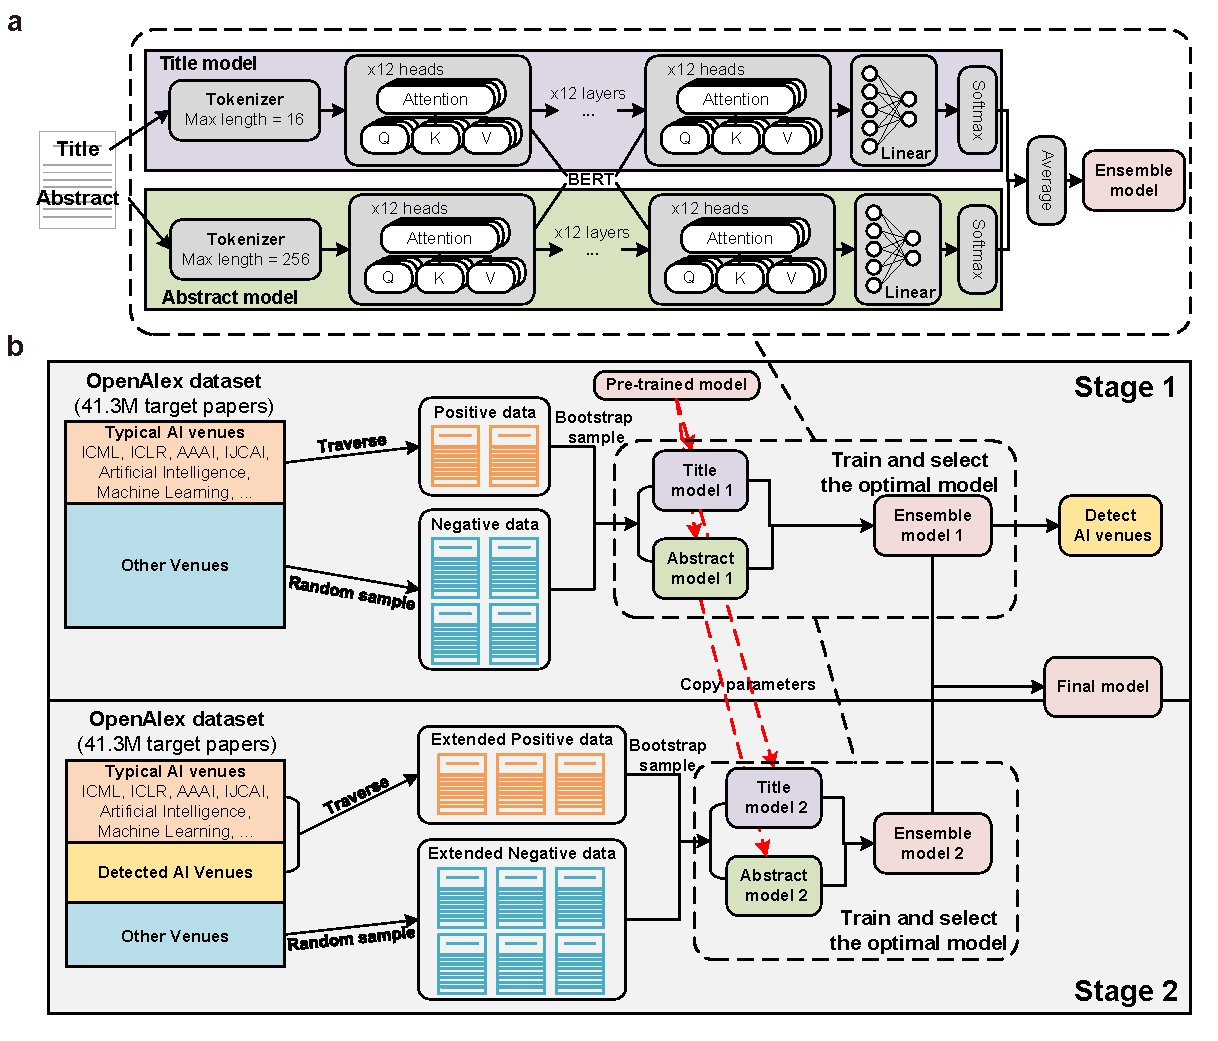
\includegraphics[width=\textwidth]{figure_ED/SD1.pdf}
\caption{
\textbf{Illustration for the method of identifying AI usage in research papers with fine-tuned language models.}
\textbf{(a)} Structure of our deployed language model, which consists of the tokenizer, the core BERT model, and the linear layer.
\textbf{(b)} Procedure of the two-stage model fine-tuning process, where we design specific approaches for constructing positive and negative data at each stage.
}
\label{figSD1}
\end{figure}

\clearpage
\begin{figure}[ht]
\centering
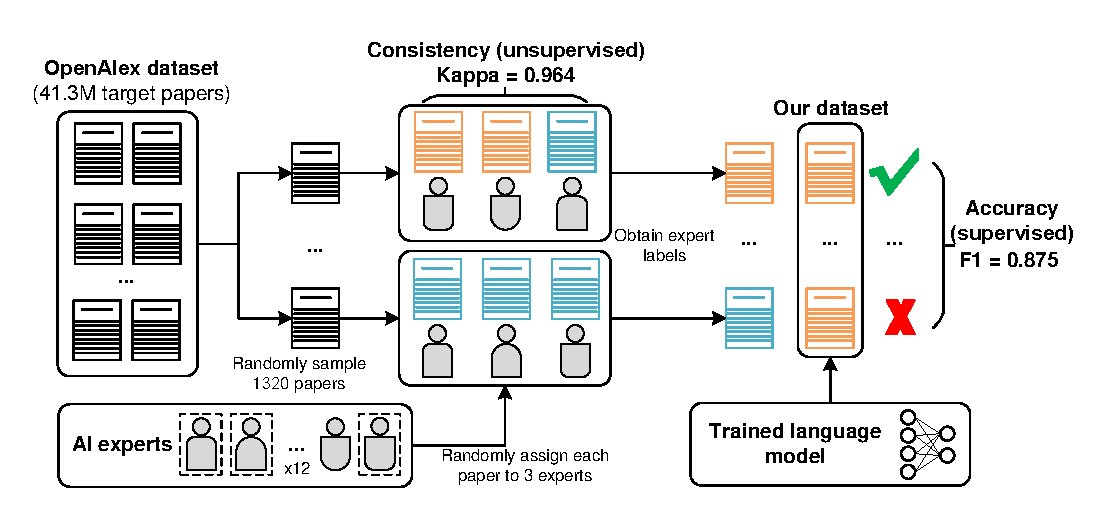
\includegraphics[width=\textwidth]{figure_ED/SD2.pdf}
\caption{
\textbf{Procedure of accuracy evaluation via expert evaluation.}
We randomly sample 1320 papers and delegate three experts to scrutinize the identification results for each paper.
We then draw the final expert label of each paper from the three experts according to the principle of the minority obeying the majority and validate the result of the language model with it.
Results indicate strong consistency among experts and high accuracy with our identification results.
}
\label{figSD2}
\end{figure}

\clearpage
\newpage
\begin{figure}[ht]
\centering
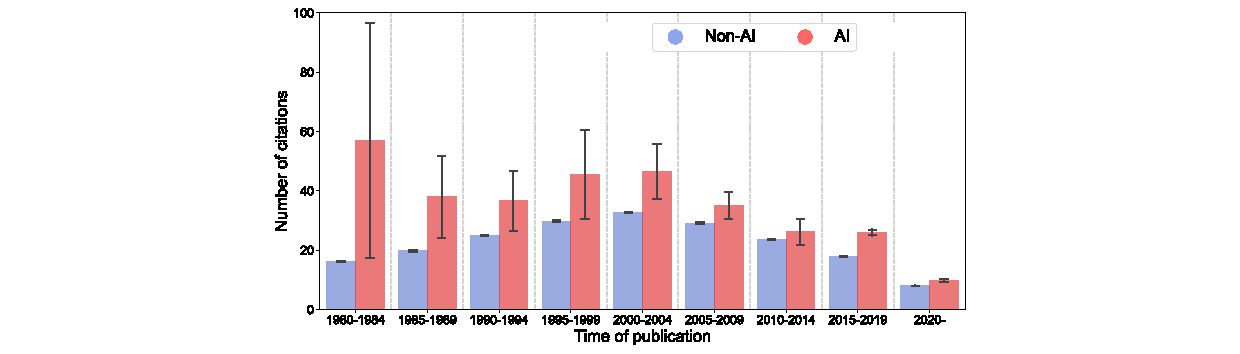
\includegraphics[width=\textwidth]{figure_ED/S2.pdf}
\caption{
\textbf{Comparison of the total citations of AI and non-AI papers published in different eras.}
The results show that AI papers consistently attract more citations over different eras ($p < 0.001, n=27,405,011$), indicating a higher academic impact than non-AI papers.
99\% CIs are shown as error bars centred at the mean, and the statistical tests use a two-sided t-test.
}
\label{figs2}
\end{figure}

\clearpage
\newpage
\begin{figure}[ht]
\centering

\includegraphics[width=\textwidth]{figure_ED/S3.pdf}
\caption{
\textbf{Annual publications of researchers adopting AI and their counterparts without AI.}
Results show that in all 6 scientific disciplines, researchers adopting AI are more productive than their counterparts without AI ($p < 0.001, n=5,377,346$).
On average, researchers adopting AI annually publish 3.02 times more papers compared with those not using AI.
99\% CIs are shown as error bars centred at the mean, and the statistical tests use a two-sided t-test.
}
\label{figs3}
\end{figure}

\clearpage
\newpage
\begin{figure}[ht]
\centering
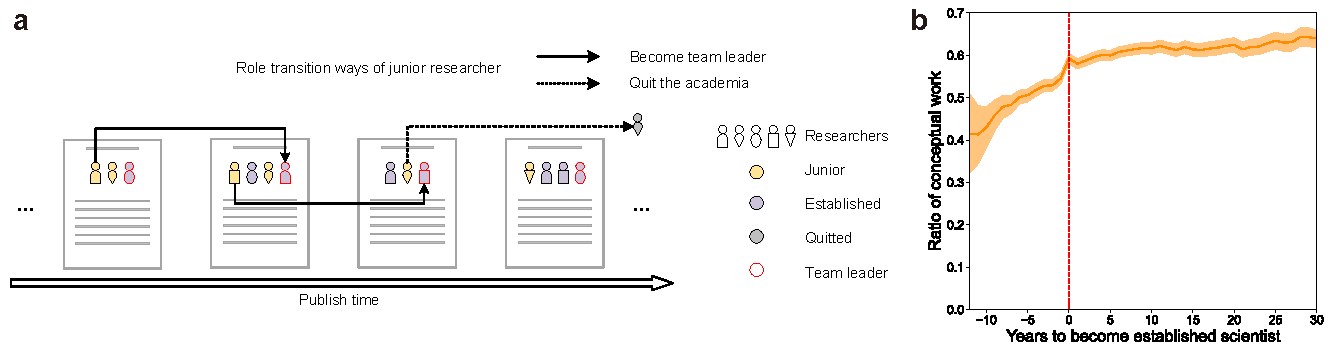
\includegraphics[width=\textwidth]{figure_ED/S4.pdf}
\caption{
\textbf{Scientists’ career role transition.}
\textbf{(a)} The career role transition of researchers.
We consider the last author of each paper as research project leader and researchers who have been research project leaders as established researchers.
Researchers who have yet to lead a research project are junior researchers, and they have two potential role transition pathways in the future: (1) become established researchers (solid arrow), and (2) abandoning academia (dashed arrow).
\textbf{(b)} Change in the ratio of conceptual work across the research career, before and after becoming an established researcher.
The ratio increases rapidly before the role transition to established researchers, while it remains stable and high after that transition.
99\% CIs are shown as error bands centred at the mean.
}
\label{figs4}
\end{figure}

\clearpage
\newpage
\begin{figure}[ht]
\centering
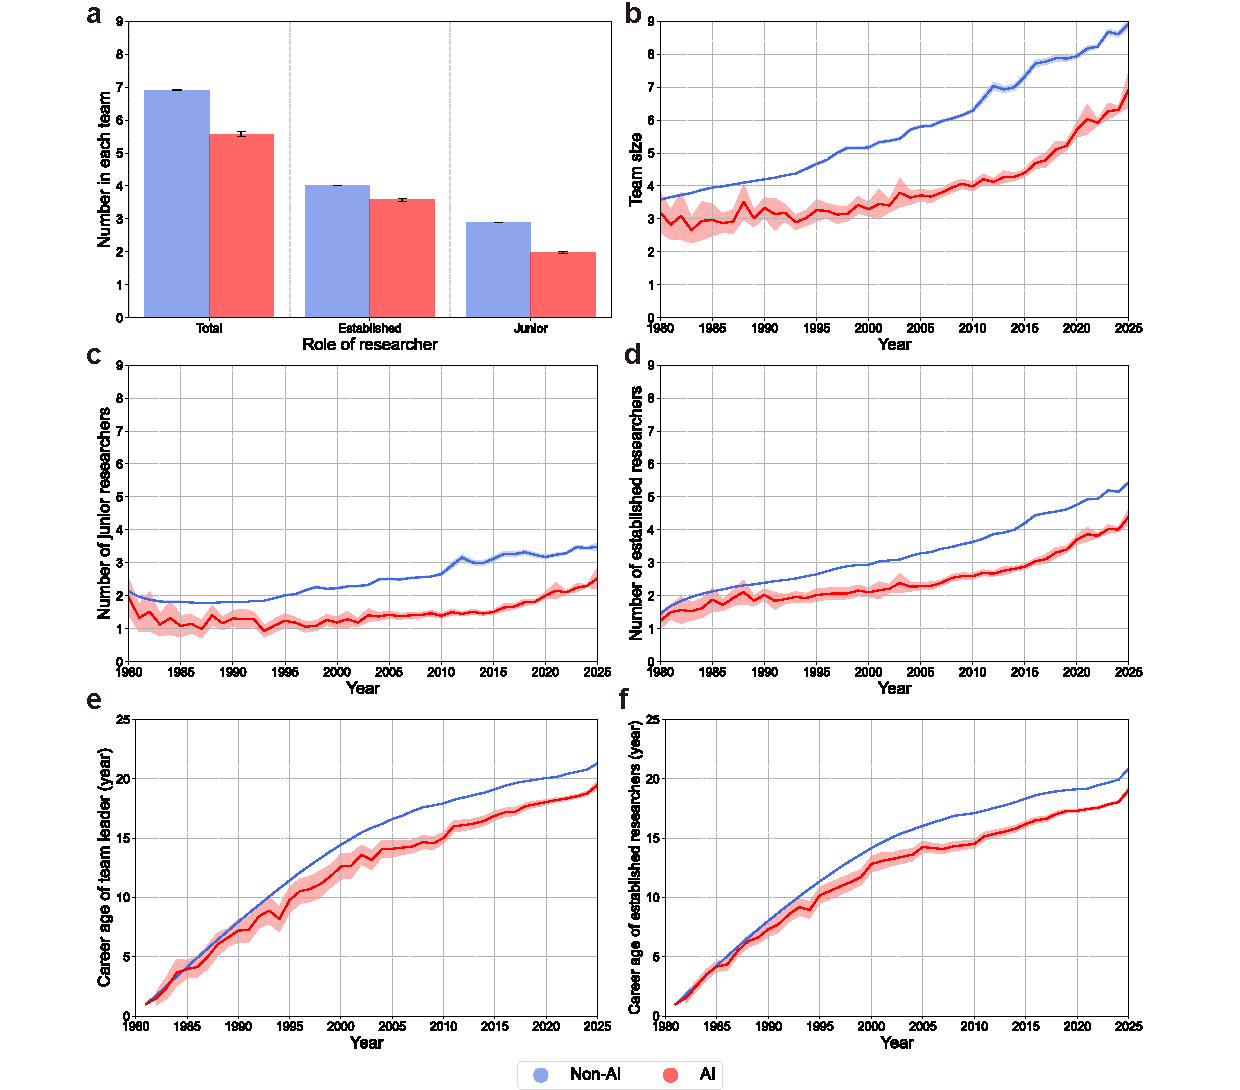
\includegraphics[width=\textwidth]{figure_ED/S5.pdf}
\caption{
\textbf{Team composition of AI and non-AI papers.}
\textbf{(a)} AI research is associated with reduced research team sizes, averaging 1.33 fewer scientists ($p<0.001, n=33,528,469$).
Specifically, the average number of junior scientists decreased from 2.89 in non-AI teams to 1.99 in AI teams (31.14\%), while the number of established scientists decreased from 4.01 to 3.58 (10.77\%).
\textbf{(b)-(d)} Change in team size, average number of junior researchers, and average number of established researchers.
These findings indicate that within the overall trend of increasing size of scientific research teams, AI adoption primarily contributes to a reduction in the number of junior scientists in teams, while a decrease in the number of established scientists is more moderate.
\textbf{(e)} The average career age of team leaders in AI and non-AI papers.
\textbf{(f)} The average career age of all involved established researchers in AI and non-AI papers.
Results indicate that AI accelerates the transition from junior to established scientists, enabling AI-adopted researchers to become established at a younger age than those without AI.
For all panels, 99\% CIs are shown as error bars or error bands centred at the mean.
All statistical tests use a two-sided t-test.
}
\label{figs5}
\end{figure}

\clearpage
\newpage
\begin{figure}[ht]
\centering
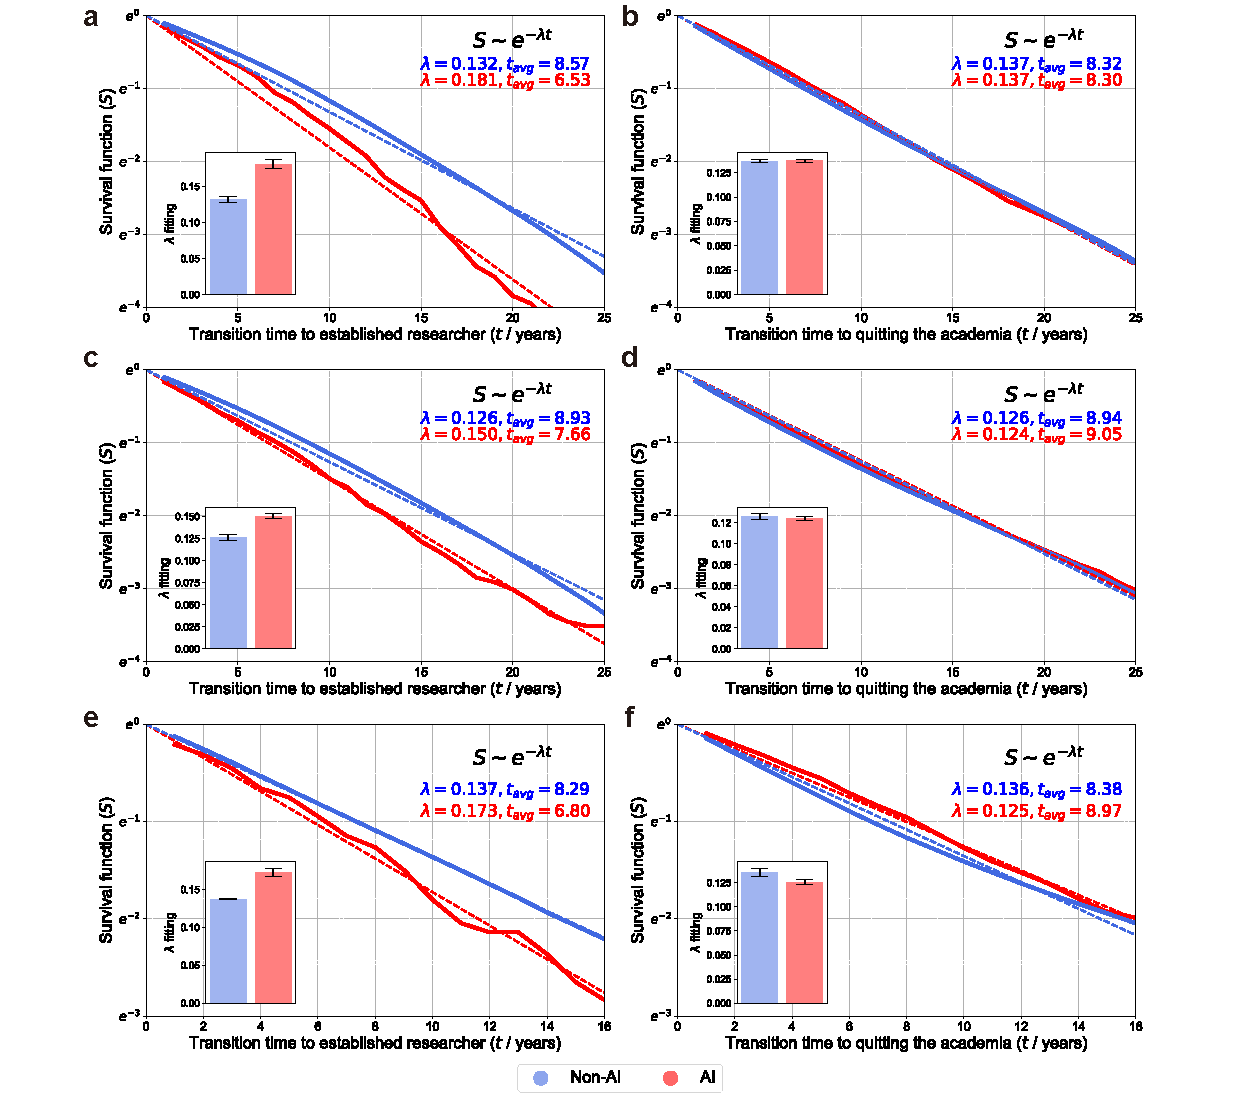
\includegraphics[width=\textwidth]{figure_ED/S6.pdf}
\caption{
\textbf{Model fitting the role transition time of junior scientists.}
\textbf{(a) (c) (e)} Survival functions for the transition from junior to established researcher in biology ($n=625,093$), medicine ($n=1,137,076$), and physics ($n=120,366$).
\textbf{(b) (d) (f)} Survival functions for the transition from junior researcher to leave academia in biology ($n=625,093$), medicine ($n=1,137,076$), and physics ($n=120,366$).
All survival function can be well-fit with exponential distributions, where the expected time for junior scientists to become established is shorter for those who adopt AI ($p<0.001$), while the expected time for junior scientists to abandon academia is similar or slightly longer for those who adopt AI.
Results indicate that AI not only provides junior scientists opportunities to become established scientists at a younger age, but also reduces the risk of their exiting academia early.
For all panels, 99\% CIs are shown as error bars centred at the mean.
All statistical tests use a two-sided t-test.
}
\label{figs6}
\end{figure}

\clearpage
\newpage
\begin{figure}[ht]
\centering
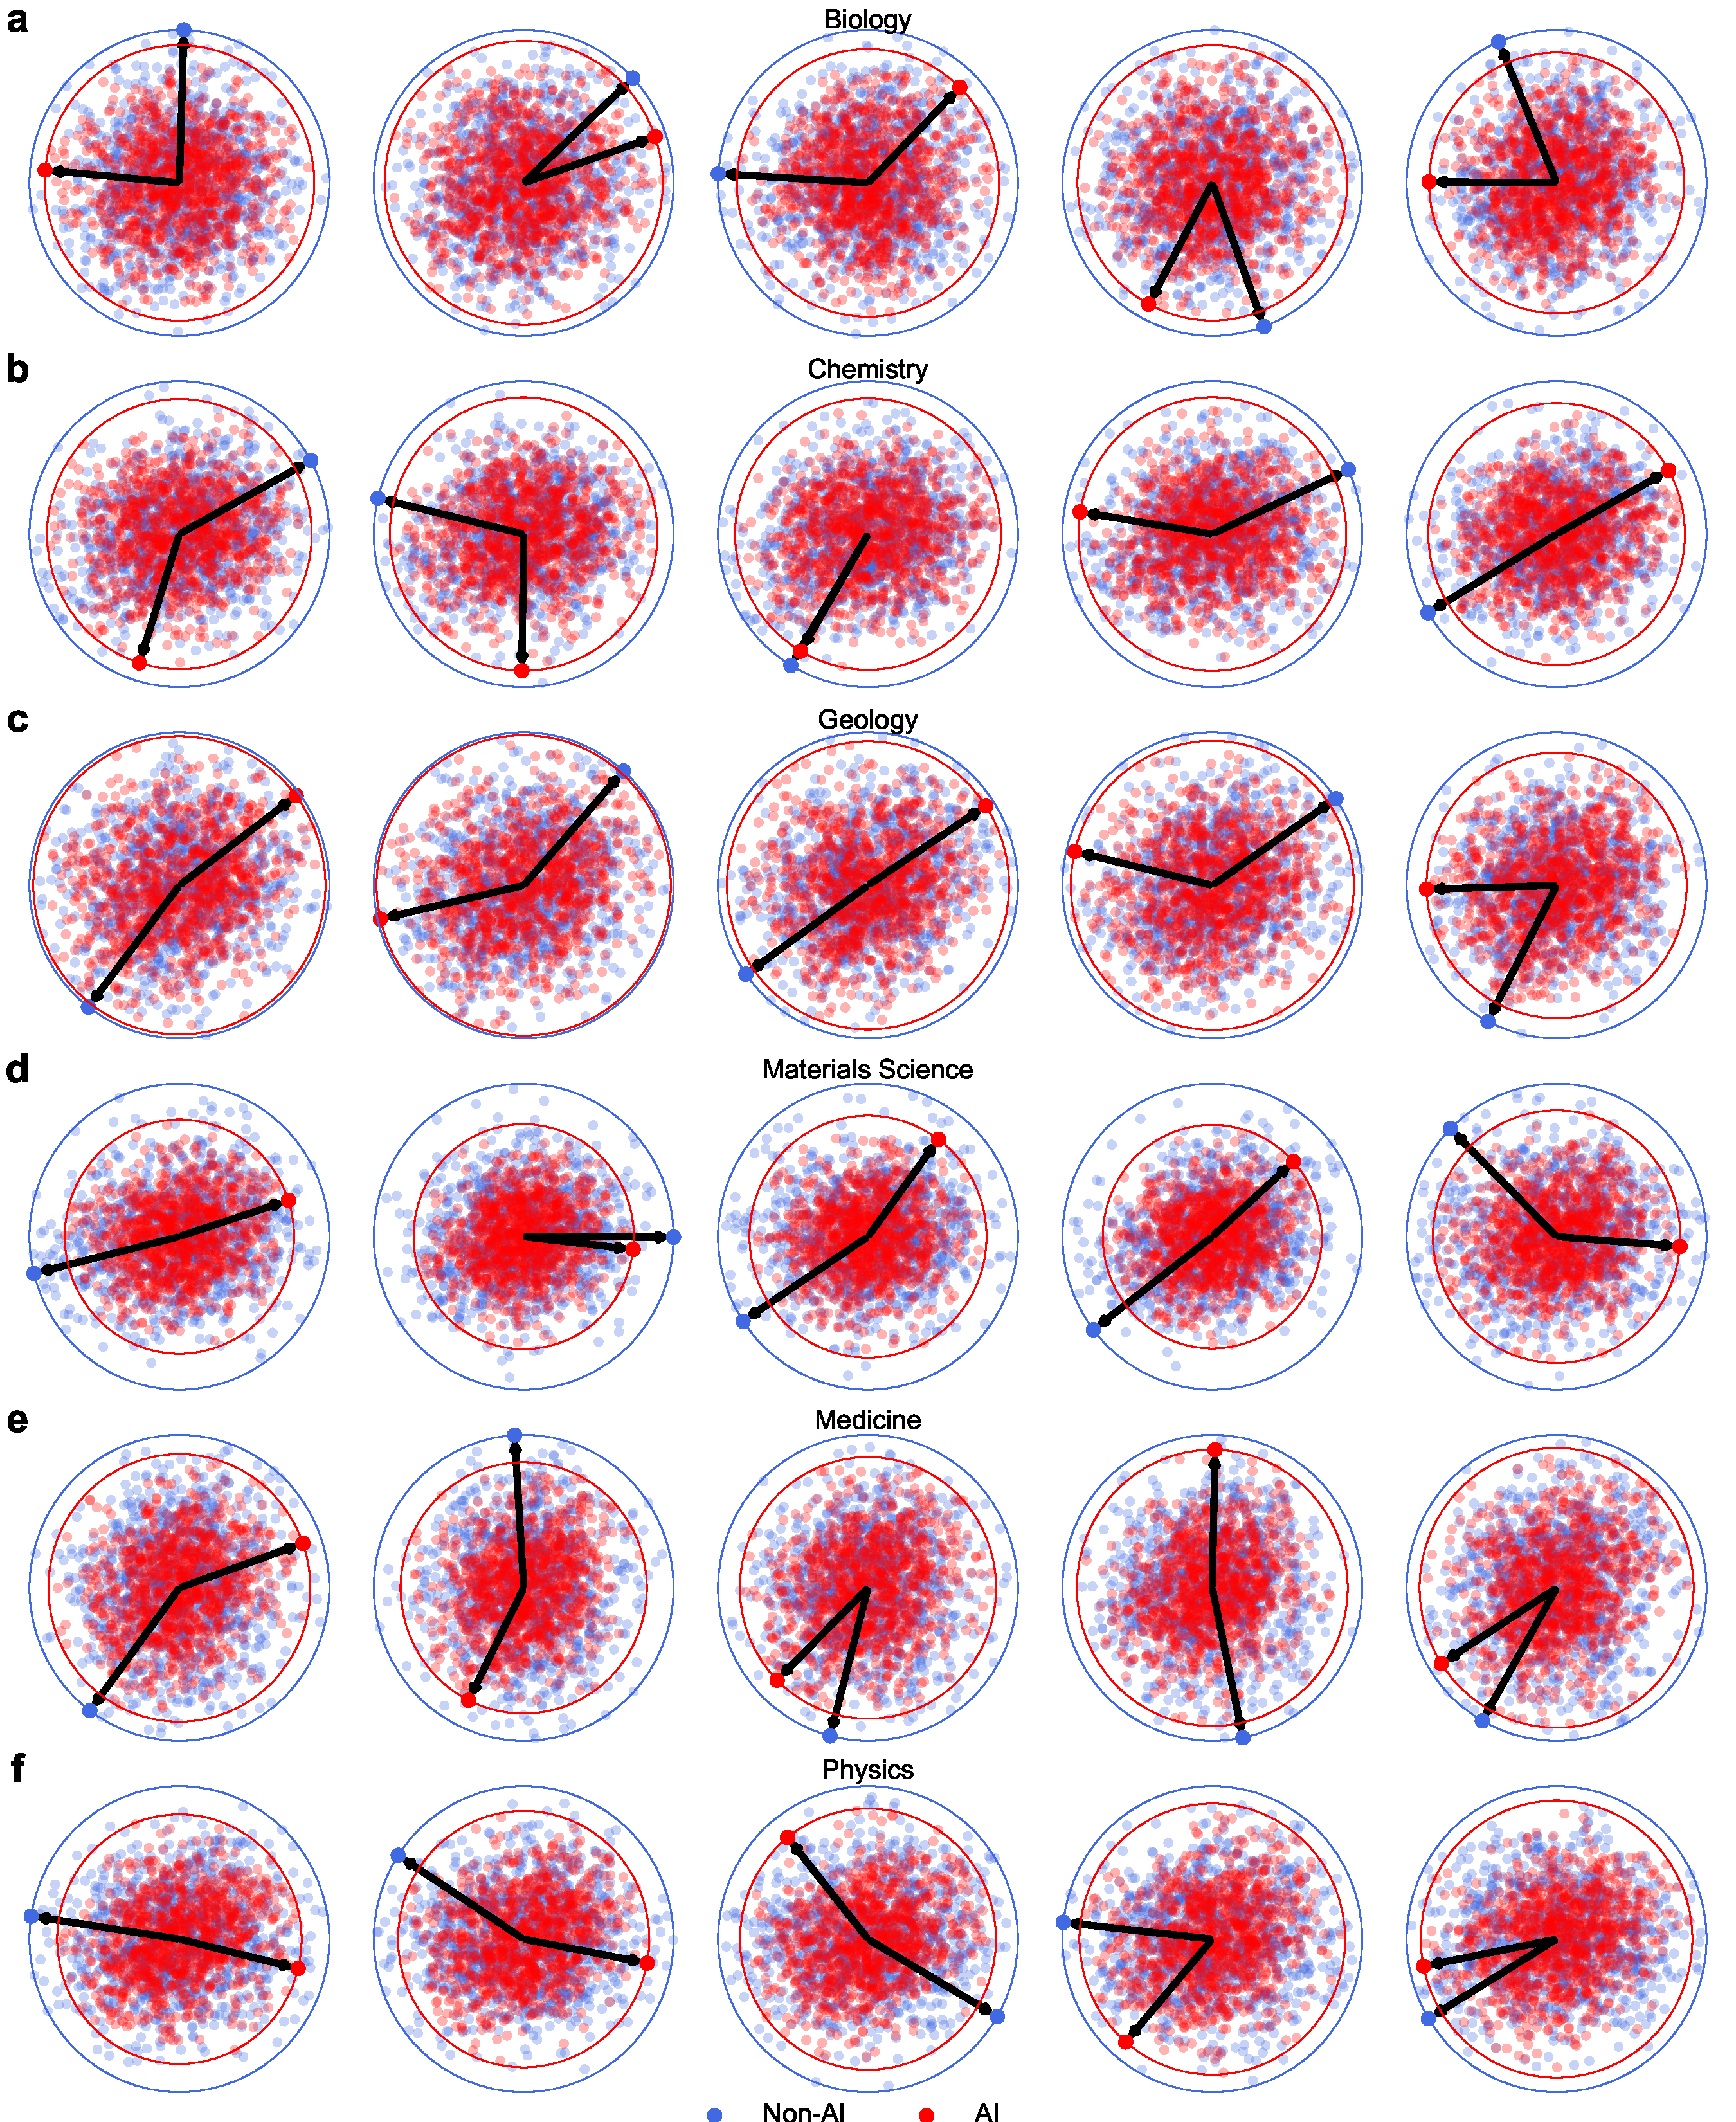
\includegraphics[width=0.8\textwidth]{figure_ED/S8.pdf}
\caption{
\textbf{The knowledge extent of AI and non-AI papers.}
Here we visualize the embeddings of a small random sample of 2,000 papers, half of which are AI papers and half are non-AI papers.
To eliminate randomness introduced by the T-SNE algorithm, here we simply pick out the first two dimensions of the high-dimensional embeddings to flatten them into a 2-D plot, and we provide 5 different random batches for each field to ensure robustness.
As shown by the solid arrows and circular boundaries, the knowledge extent of AI papers is smaller than that of a comparable sample of non-AI papers, which is consistent across the fields studied in our analysis.
}
\label{figs8}
\end{figure}

\clearpage
\newpage
\begin{figure}[ht]
\centering
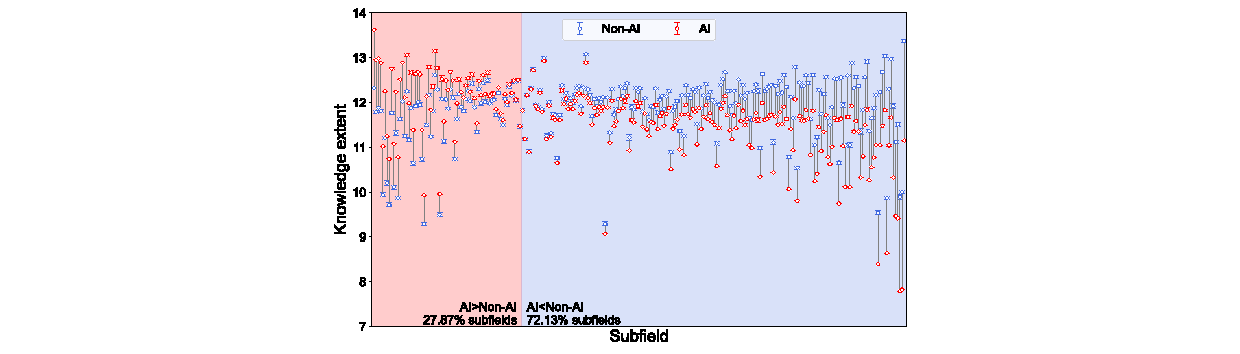
\includegraphics[width=\textwidth]{figure_ED/S9.pdf}
\caption{
\textbf{The knowledge extent of AI and non-AI papers in each subfield.}
Compared with conventional research, AI research is associated with a shrinkage in the collective knowledge extent of science, where the contraction of knowledge extent can be observed in more than 70\% of over two hundred sub-fields ($n=1,000$ samples in each subfield).
For all subfields, 99\% CIs are shown as error bars centred at the mean.
}
\label{figs9}
\end{figure}

\clearpage
\newpage
\begin{figure}[ht]
\centering
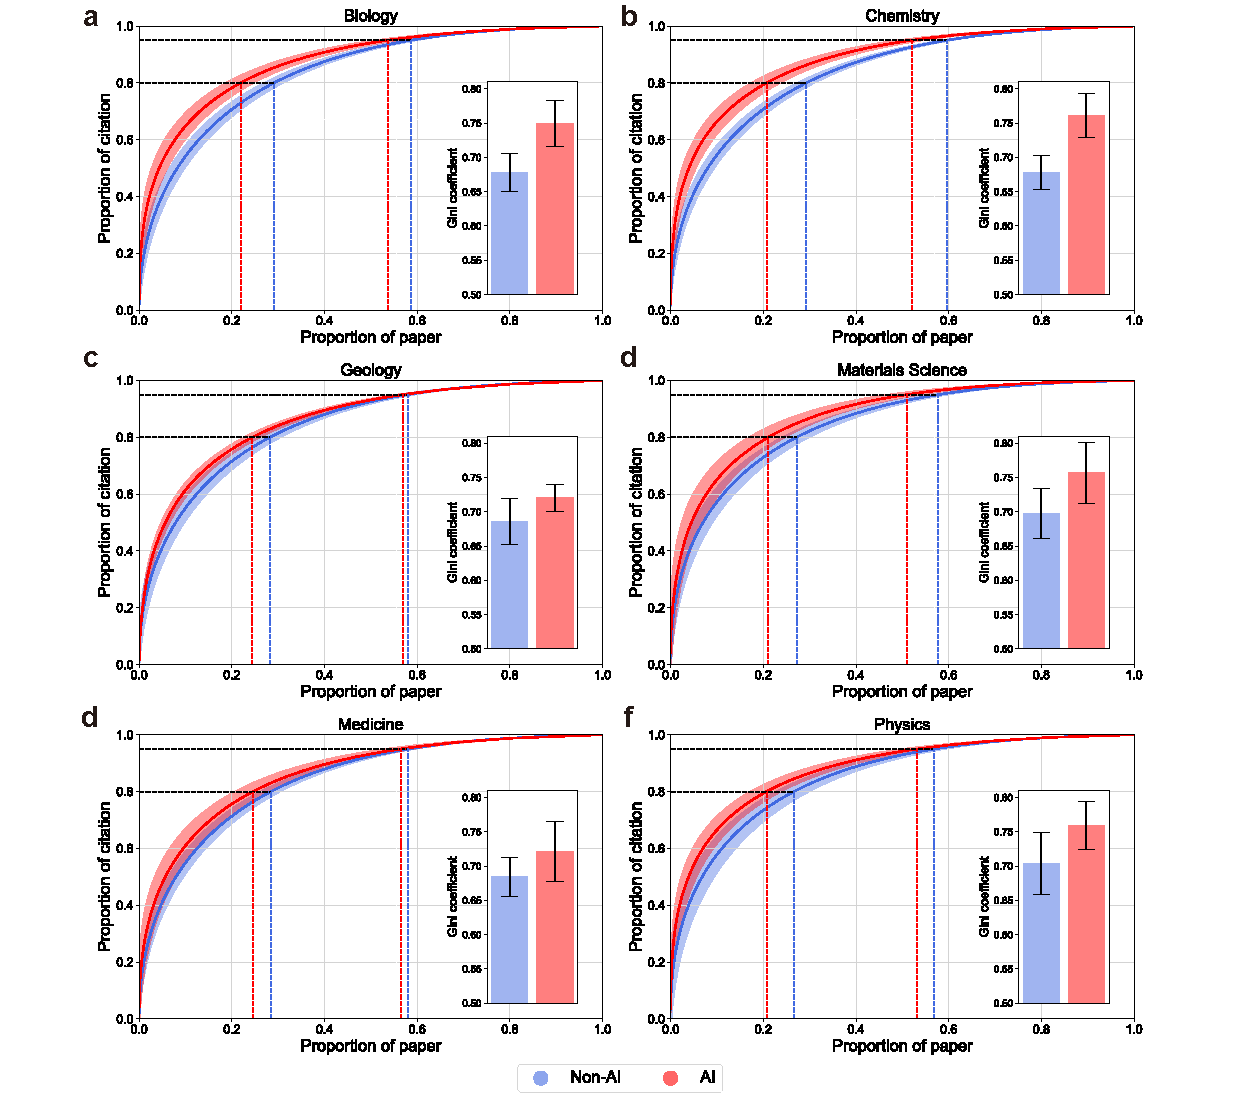
\includegraphics[width=\textwidth]{figure_ED/S10.pdf}
\caption{
\textbf{The Matthew effect in citations to AI and non-AI papers.}
In AI research, a small number of superstar papers dominate the field, with approximately 20\% of top papers receiving 80\% of citations and 50\% receiving 95\%.
This unequal distribution leads to a higher GINI coefficient in citation patterns surrounding AI research ($p<0.001, n=100$ sampled paper groups for each discipline).
Such disparity in the recognition of AI papers is consistent across all fields examined.
For all panels, 99\% CIs are shown as error bars or error bands centred at the mean.
All statistical tests use a two-sided t-test.
}
\label{figs10}
\end{figure}